\documentclass[a4paper,10pt]{article}
\usepackage{fullpage}
\usepackage{float}
\usepackage[english]{babel}
\usepackage{graphicx,subfig,wrapfig}
\usepackage{amsmath,amsfonts,amsthm,amssymb}
\usepackage{fancyhdr,fancybox,color}
\usepackage{enumerate}
\usepackage[amssymb]{SIunits}
\definecolor{MyBlue}{rgb}{0,0.3,0.6}
\usepackage[colorlinks=true,
linkcolor=MyBlue,
plainpages=false,
citecolor=MyBlue,
urlcolor=MyBlue]{hyperref}
\usepackage[all]{hypcap}
\usepackage[url=false,
backend=bibtex,
style=authoryear-comp,
doi=true,
isbn=true,
backref=false,
dashed=false,
maxcitenames=2,
maxbibnames=99,
natbib=true]{biblatex}
\DeclareNameAlias{author}{last-first}
\renewbibmacro{in:}{}
\addbibresource{refrence.bib}
\nonfrenchspacing
\begin{document}
\noindent Chair: Physics of Fluids Department
\begin{center}
 \begin{LARGE}
  Bursting of champagne bubbles: Numerics \& Experiments
 \end{LARGE}
\end{center}
\section*{Description}
If one notices carefully a glass of champagne (see figure \ref{fig:champange}) or a carbonated beverage, the air bubble in the liquid rises due to buoyancy and reaches the liquid-air interface. The bubble sits at the interface for a while and then bursts, creating a cavity in the interface. Bubble bursting like this is observed in many real-life scenarios. This process is responsible for transporting aromatics from champagne and pathogens from contaminated water. Furthermore, bubbles bursting in oceans emit nuclei that are essential for cloud formation in our atmosphere. 

The newly formed cavity desires to flatten out due to surface tension effects, and capillary waves begin traveling to serve this purpose. However, traveling waves do more than flatten the cavity; they collide at the bottom of the cavity, creating a jet that breaks into vertically projected droplets; see figures \ref{Figure::Typical} \& \ref{Figure::Waves}. This phenomenon has been widely studied by \citet{duchemin2002jet, walls2015jet, deike2018dynamics, gordillo2019capillary}.

Nonetheless, we lack a comprehensive understanding of the influence of liquid properties, especially non-Newtonian effects of surrounding liquid on the overall dynamics. Bubble-bursting in non-Newtonian media is observed in several geophysical phenomena such as mudpots (see \citet{sanjay_lohse_jalaal_2021} and \href{https://www.youtube.com/watch?v=a9hUsVq9q7U}{YouTube link}). In addition to its practical applications, bubble-bursting in non-Newtonian medium has great scientific relevance. For instance, understanding the bubble-bursting dynamics in a viscoelastic medium teaches us a great deal and paves the way for understanding much more complex flows, such as coughing or sneezing. Such a phenomenon involves the breaking of mucosalivary fluids (which shows viscoelastic behavior) into droplets that are primarily responsible for airborne disease transmission \citep{walls2017quantifying, bourouiba2021fluid}. You will numerically study the dynamics produced by bubble bursting in a viscoelastic medium (see \citet{dixit2024viscoelastic}). The numerical results obtained will be compared with the experimental findings from a parallel project. Finally, the implication of our analysis will be made on the understanding of droplet distribution during coughing or sneezing. 

\begin{figure}[H]
	\begin{center}
		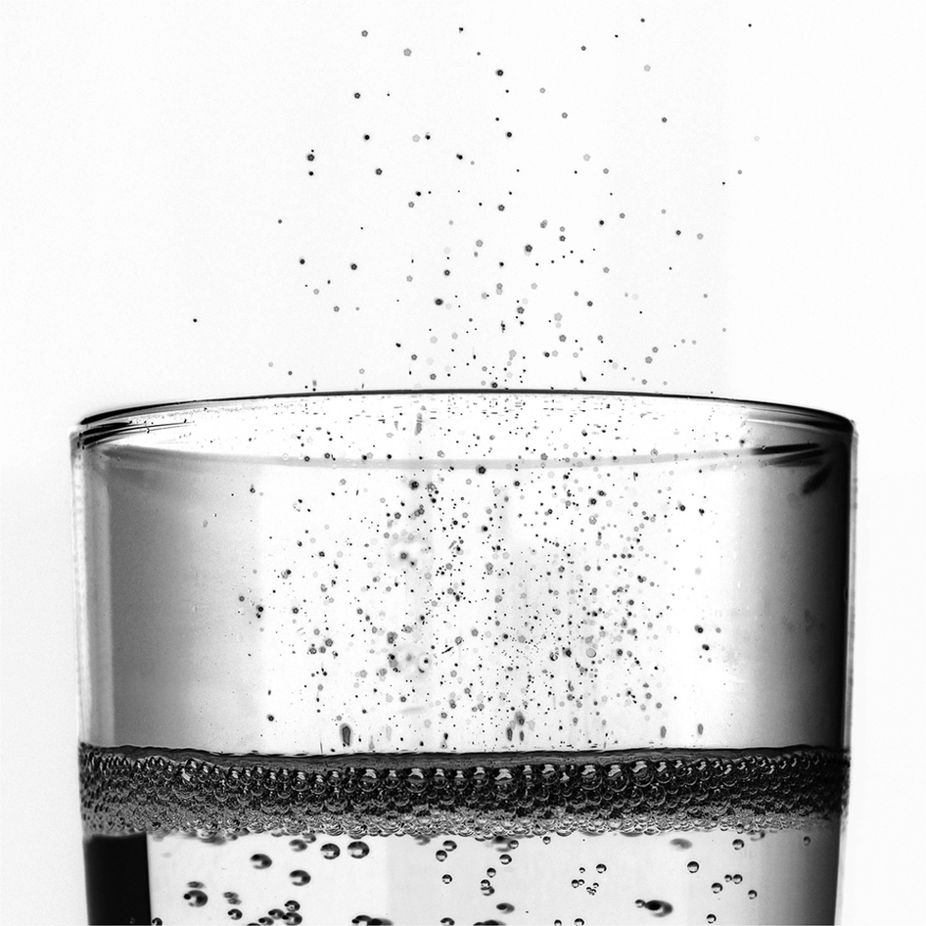
\includegraphics[width=0.4\textwidth]{champagne.jpg}
		\caption{\citet{ghabache2016evaporation} reported the collapse of numerous bubbles at the free surface, emitting a cloud of tiny droplets, which is characteristic of champagne and other sparkling wines and enhances the sensual experience of the taster.}
		\label{fig:champange}
	\end{center}
\end{figure}

\begin{figure}[H]
\begin{center}
 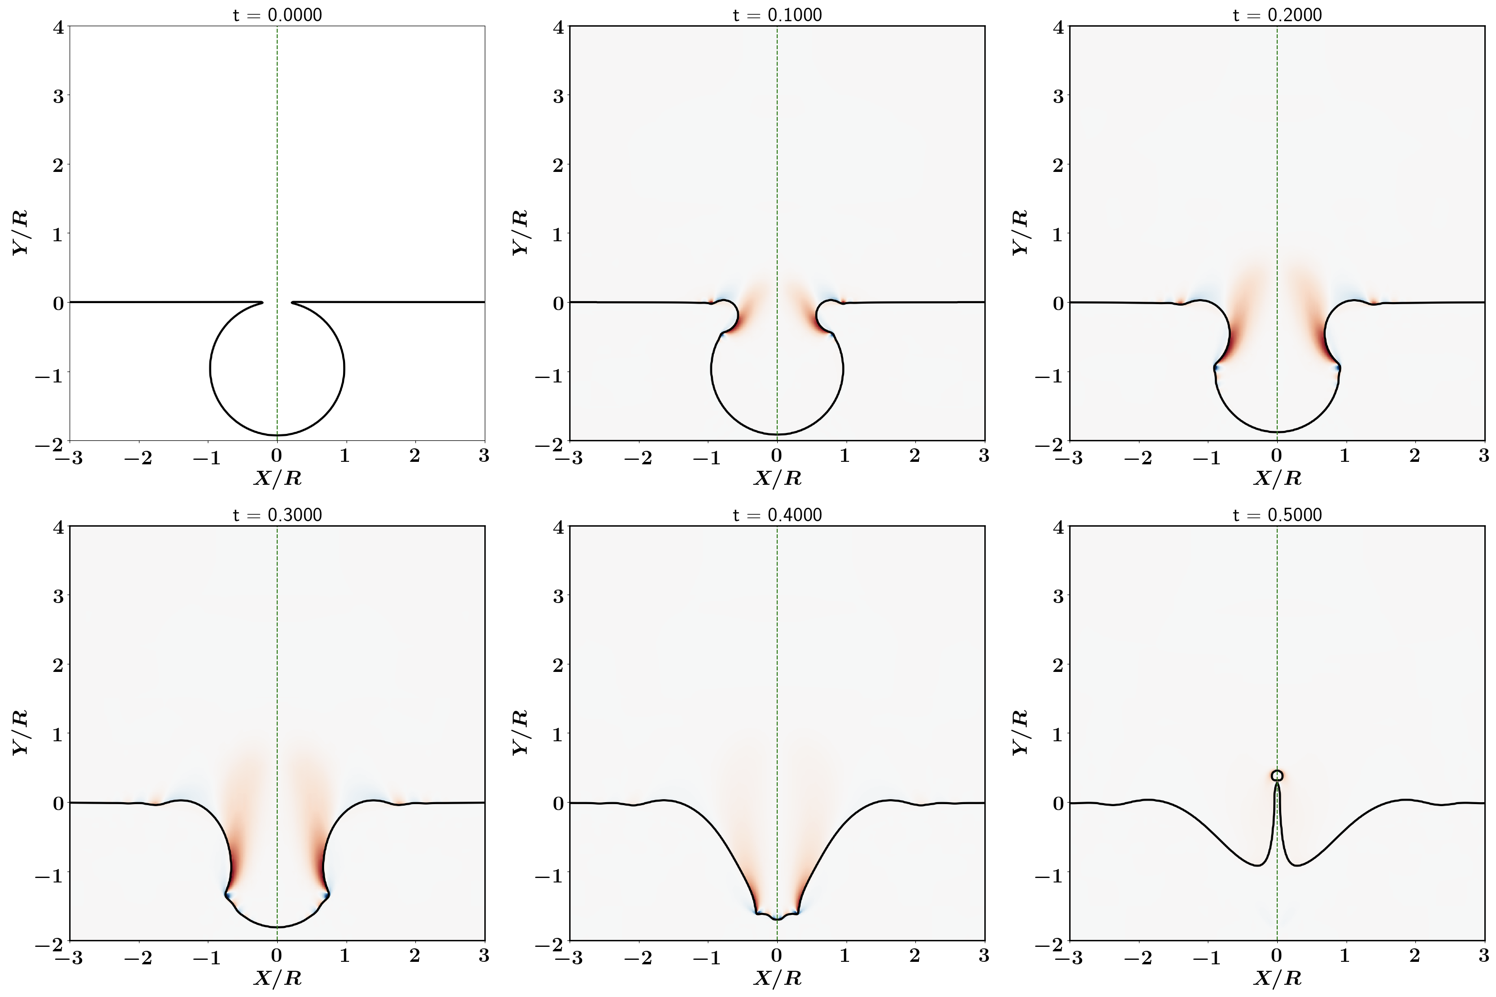
\includegraphics[width=0.95\textwidth]{temporal.png}
 \caption{Time evolution of the dynamics of open bubble cavity at the water surface. The color shows the magnitude of non-dimensionalized vorticity, $\Gamma$ (maximum $\Gamma$ = 150 with red and minimum $\Gamma$ = -150 with blue).}
 \label{Figure::Typical}
\end{center}
\end{figure}


\begin{figure}[H]
\begin{center}
 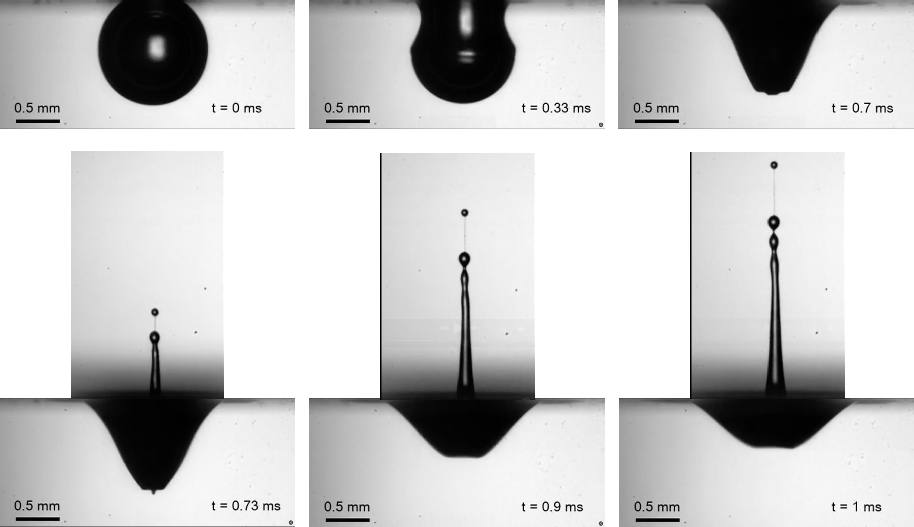
\includegraphics[width=0.95\textwidth]{schematic.pdf}
 \caption{Observation of the time evolution of the open bubble cavity. The lower rows display two views: the top view is above the water surface, while the bottom view is below the surface. }
 \label{Figure::Waves}
\end{center}
\end{figure}
\section*{What you will do and what you will learn?}

\begin{enumerate}
\item You will learn about the physics of fluids, and science underlying non-Newtonian fluid flows. 
\item You will learn how to utilize state-of-the-art computational tools to study real life physics. 
\item You will have access to a read-to-use codebase (available on \href{https://github.com/comphy-lab/Viscoelastic-Worthington-jets-and-droplets-produced-by-bursting-bubbles}{GitHub}).
\item As a part of the \href{https://comphy-lab.org}{CoMPhy lab} at the Physics of Fluids Dept., you will learn and adapt open-source coding principles. 
\item You will learn how to collaborate with a diverse group of researchers, specifically with other numericists, experimentalists and theoreticians.

\end{enumerate}

If you have any questions, feel free to contact \href{mailto:a.k.dixit@utwente.nl}{Ayush} (details below).
\begin{center}
\begin{tabular}{|l|l|l|}
\hline \textbf{Supervision} & \textbf{E-mail} & \textbf{Office} \\
\hline Ayush Dixit & \href{mailto:a.k.dixit@utwente.nl}{a.k.dixit@utwente.nl} & Meander 250 \\
\hline Coen Verschuur & \href{mailto:c.i.verschuur@utwente.nl}{c.i.verschuur@utwente.nl} & Meander 114B \\
\hline Dr. Vatsal Sanjay & \href{mailto:vatsalsy@comphy-lab.org}{vatsalsy@comphy-lab.org} & Meander 246B \\
\hline Dr. Alexandros Oratis   & \href{mailto:a.t.oratis@utwente.nl}{a.t.oratis@utwente.nl}& TU Delft \\
\hline Prof. Dr. Detlef Lohse & \href{mailto:d.lohse@utwente.nl}{d.lohse@utwente.nl} & Meander 261  \\
\hline
\end{tabular}
\end{center}
\printbibliography
\end{document}
